\documentclass[a4paper]{article}
\usepackage[T1]{fontenc}
\usepackage[utf8]{inputenc}
\usepackage{lmodern}
\usepackage{amsmath,amssymb}
\usepackage[top=3cm,bottom=2cm,left=2cm,right=2cm]{geometry}
\usepackage{fancyhdr}
\usepackage{esvect}
\usepackage{xcolor}
\usepackage{tikz}\usetikzlibrary{calc}

\parskip 1em\parindent 0pt

\begin{document}

\pagestyle{fancy}
\fancyhf{}
\setlength{\headheight}{15pt}
\fancyhead[L]{Optique}\fancyhead[R]{Question 7}

% Énoncé
\begin{center}
	\large{\boldmath{\textbf{Différence de marche et interfrange \\ pour les trous d’Young avec lentille de projection}}}
\end{center}

% Correction

\begin{center}
	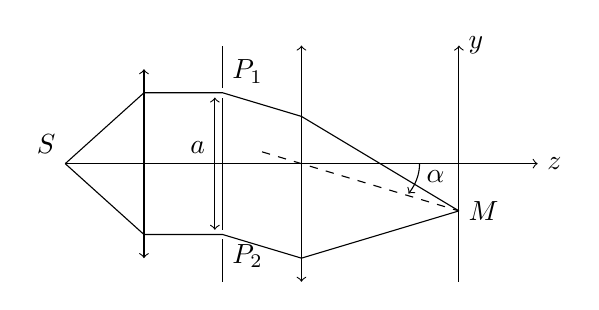
\begin{tikzpicture}[yscale=.6]
    \draw[->] (0,0) node[above left]{$S$} to (6,0) node[right]{$\vv z$};
    \draw[<->] (1,-2) -- (1,2);
    \draw [<->] (1.9,1.4)--(1.9,-1.4);
    \draw (1.9,0) node [anchor=south east]{$a$};
    \draw (2,0) -- (2,1.4) (2,1.6) -- (2,2.5);
    \draw (2,0) -- (2,-1.4) (2,-1.6) -- (2,-2.5);
    \draw[->] (5,-2.5) -- (5,2.5) node[right]{$\vv y$};
    \draw[<->] (3,-2.5) -- (3,2.5);
    \draw (0,0) to (1,1.5) to (2,1.5) node[above right]{$P_1$} -- (3,1) -- (5,-1);
    \draw (0,0) to (1,-1.5) to (2,-1.5) node[below right]{$P_2$} -- (3,-2) -- (5,-1) node[right]{$M$};
    \draw[dashed] (2.5,.25) -- (5,-1);
    \draw[->] (4.5,0) node[below right=-1pt]{$\alpha$} arc (0:-25:1.5);
	\end{tikzpicture}
\end{center}

Par théorème de Malus, \( \delta = a \cdot \sin(\alpha) \) or \(\tan(\alpha) = \dfrac{x}{f'}\).\\
On se trouve dans les conditions de Gauss donc \( \alpha \ll 1 \).\\
\fcolorbox{red}{white}{D'où \( \delta = \dfrac{a x}{f'}\)}
\par

Par définition de l'interfrange, \( p(x + i) = p(x) \) d'où \( \dfrac{a i}{\lambda f'} = 1 \).\\
\fcolorbox{red}{white}{Donc \(i = \dfrac{\lambda f'}{a} \)}


\end{document}
